%%%%%%%%%%%%%%%%%%%%%%%%%%%%%%%%%%%%%%%%%
% Beamer Presentation
% LaTeX Template
% Version 1.0 (10/11/12)
%
% This template has been downloaded from:
% http://www.LaTeXTemplates.com
%
% License:
% CC BY-NC-SA 3.0 (http://creativecommons.org/licenses/by-nc-sa/3.0/)
%
%%%%%%%%%%%%%%%%%%%%%%%%%%%%%%%%%%%%%%%%%

%----------------------------------------------------------------------------------------
%	PACKAGES AND THEMES
%----------------------------------------------------------------------------------------

\documentclass{beamer}

\mode<presentation> {

% The Beamer class comes with a number of default slide themes
% which change the colors and layouts of slides. Below this is a list
% of all the themes, uncomment each in turn to see what they look like.

\usetheme{default}
%\usetheme{AnnArbor}
%\usetheme{Antibes}
%\usetheme{Bergen}
%\usetheme{Berkeley}
%\usetheme{Berlin}
%\usetheme{Boadilla}
%\usetheme{CambridgeUS}
%\usetheme{Copenhagen}
%\usetheme{Darmstadt}
%\usetheme{Dresden}
%\usetheme{Frankfurt}
%\usetheme{Goettingen}
%\usetheme{Hannover}
%\usetheme{Ilmenau}
%\usetheme{JuanLesPins}
%\usetheme{Luebeck}
%\usetheme{Madrid}
%\usetheme{Malmoe}
%\usetheme{Marburg}
%\usetheme{Montpellier}
%\usetheme{PaloAlto}
%\usetheme{Pittsburgh}
%\usetheme{Rochester}
%\usetheme{Singapore}
%\usetheme{Szeged}
%\usetheme{Warsaw}

% As well as themes, the Beamer class has a number of color themes
% for any slide theme. Uncomment each of these in turn to see how it
% changes the colors of your current slide theme.

%\usecolortheme{albatross}
%\usecolortheme{beaver}
%\usecolortheme{beetle}
%\usecolortheme{crane}
%\usecolortheme{dolphin}
%\usecolortheme{dove}
%\usecolortheme{fly}
%\usecolortheme{lily}
%\usecolortheme{orchid}
%\usecolortheme{rose}
%\usecolortheme{seagull}
%\usecolortheme{seahorse}
%\usecolortheme{whale}
%\usecolortheme{wolverine}

\useoutertheme{infolines}

\usepackage[official]{eurosym}
\usepackage{svg}
\usepackage{amsmath}
\usepackage{graphicx}
\usepackage{multirow}
\usepackage[utf8]{inputenc}
\usepackage{subfig}
\usepackage{listings}
\usepackage{outlines}
\usepackage[noend]{algorithm,algorithmic}
\usepackage{caption}
\usepackage{setspace}
\usepackage{threeparttable}



%\setbeamertemplate{footline} % To remove the footer line in all slides uncomment this line
%\setbeamertemplate{footline}[page number] % To replace the footer line in all slides with a simple slide count uncomment this line

%\setbeamertemplate{navigation symbols}{} % To remove the navigation symbols from the bottom of all slides uncomment this line
}

\usepackage{graphicx} % Allows including images
\usepackage{booktabs} % Allows the use of \toprule, \midrule and \bottomrule in tables

%----------------------------------------------------------------------------------------
%	TITLE PAGE
%----------------------------------------------------------------------------------------

\title[BPP]{Bin Packing Problem:\\ A general purpose Hill Climbing procedure } % The short title appears at the bottom of every slide, the full title is only on the title page


 % Your name
\institute[FSU-Jena] % Your institution as it will appear on the bottom of every slide, may be shorthand to save space
{ 
Seminar Modern Heuristics \\
Dr. Rico Walter
}

\author{Lukas Schmauch, Sebastian Wolf}
\date{Februar 2021} % Date, can be changed to a custom date

\begin{document}
\begin{frame}
\titlepage % Print the title page as the first slide
\end{frame}
%-------------------------------------
\begin{frame}
\frametitle{Übersicht} 
\tableofcontents
\end{frame}

%----------------------------------------------------------------------------------------
%	PRESENTATION SLIDES

%%%------------------------------------------------
\section{Was ist das Bin Packing Problem?} 
\begin{frame}
\frametitle{Bin Packing Problem - Kurzübersicht}
\begin{footnotesize}
\begin{itemize}
\item Geg. eine Menge $\varphi$ mit $n$ unterschiedlichen Items
\item Ziel: Konstruiere die Menge $U=\{U_1,...,U_G\}$, wobei:
\item[]
\item Alle Items müssen verpackt werden
\item[] $\cup U_i = \varphi \ (for \ i = 1,...,G)$
\item[]
\item Bins enthalten nie das gleiche Item
\item[] $U_i \cap U_j = \emptyset \ (for \ 1 \leq i\neq j \leq G )$
\item[]
\item Es existieren keine leeren Bins
\item[] $U_i\neq \emptyset \ (for \ i=1,...,G)$
\item[]
\end{itemize}
\end{footnotesize}
\end{frame}
%%%------------------------------------------------
\section{Hill Climbing Ansatz} 
\begin{frame}
\frametitle{Grundidee Hill Climbing Ansatz}
\begin{footnotesize}
\begin{itemize}
\item Verbesserungsverfahren mit First Fit Ansatz
\end{itemize}
\end{footnotesize}
\begin{figure}[!htbp]
\begin{center}
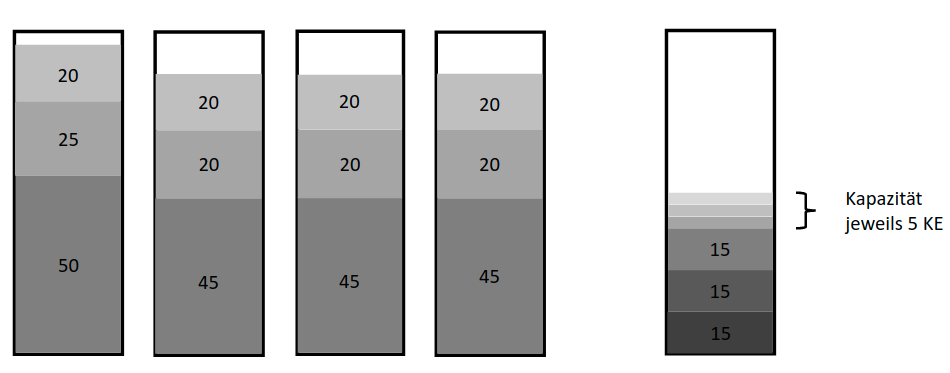
\includegraphics[scale=0.25]{img/HC_idee.png}
\end{center}
\end{figure}

\begin{scriptsize}
\begin{itemize}
\item Lewis, R. (2009): A general-purpose hill-climbing method for order independent minimum grouping problems: A case study in graph colouring and bin packing. Computers & Operations Research 36, 2295–2310.
\end{itemize}
\end{scriptsize}
\end{frame}
%%%------------------------------------------------
%%%------------------------------------------------
\begin{frame}
\frametitle{Ablauf Hill Climbing Verfahren}
\begin{footnotesize}
\begin{enumerate}
\item Eröffnungsverfahren (First Fit Descending)
\item Zufällige Auswahl von Bins 
\item Ausführung des Verbesserungsverfahrens
\item Füge Gruppen wieder zusammen
\item Shuffle der Gruppen
\item Greedy Algorithmus
\item Wiederhole Schritt 2-6 bis Abbruchkriterium erreicht
\end{enumerate}
\end{footnotesize}
\end{frame}

%%%------------------------------------------------
\begin{frame}
\frametitle{1. Eröffnungsverfahren - First Fit Descending}
\begin{itemize}
\item Sortierung nach absteigender Itemkapazität
\item Anwendung des Greedy Algorithmus
\end{itemize}
\begin{figure}[!htbp]
\begin{center}
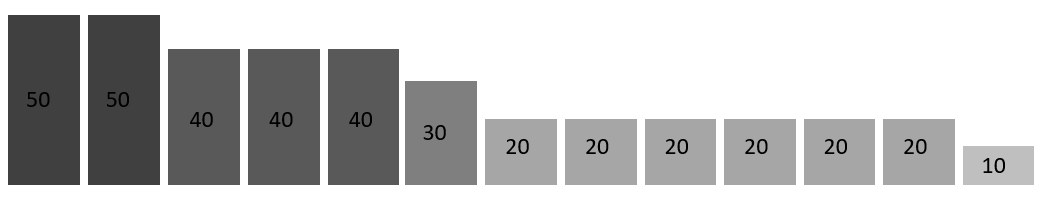
\includegraphics[scale=0.25]{img/FFD_items.png}
\end{center}
\end{figure}

\begin{figure}
\begin{center}
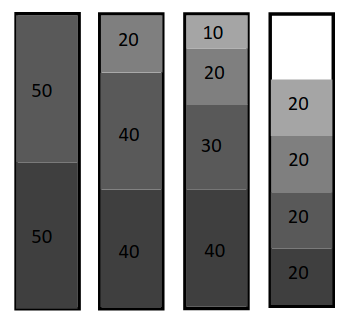
\includegraphics[scale=0.25]{img/Greedy.png}
\end{center}
\end{figure}




\end{frame}
%%%------------------------------------------------
\begin{frame}
\frametitle{2. Zufällige Auswahl von Bins}
\begin{footnotesize}
\begin{itemize}
\item \textbf{Standardverfahren:} Auswahl eines Bins mit Wahrscheinlichkeit $p=\frac{1}{\# Gruppen}$
\end{itemize}
\end{footnotesize}
\begin{figure}[!htbp]
\begin{center}
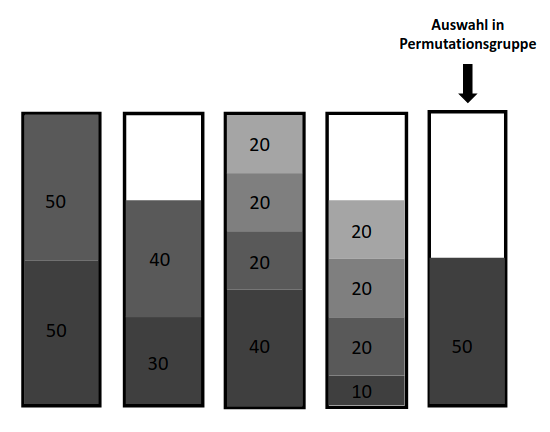
\includegraphics[scale=0.25]{img/HC_1.png}
\end{center}
\end{figure}
\begin{footnotesize}
\begin{itemize}
\item \textbf{Modifikation:} Bin mit minimaler Itemzahl
\end{itemize}
\end{footnotesize}

\end{frame}
%%%------------------------------------------------
\begin{frame}
\frametitle{3. Ausführung des Verbesserungsverfahrens}
\begin{figure}[!htbp]
\begin{center}
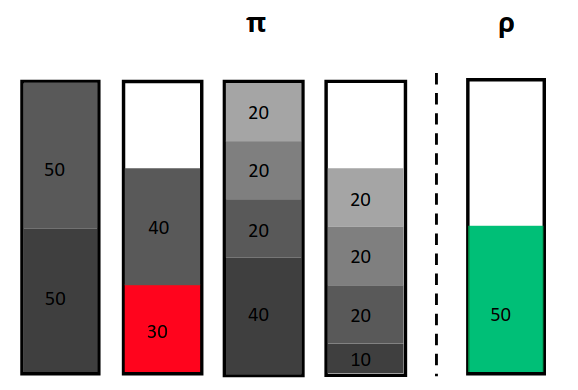
\includegraphics[scale=0.25]{img/HC_1.5.png}
\end{center}
\end{figure}

\begin{figure}[!htbp]
\begin{center}
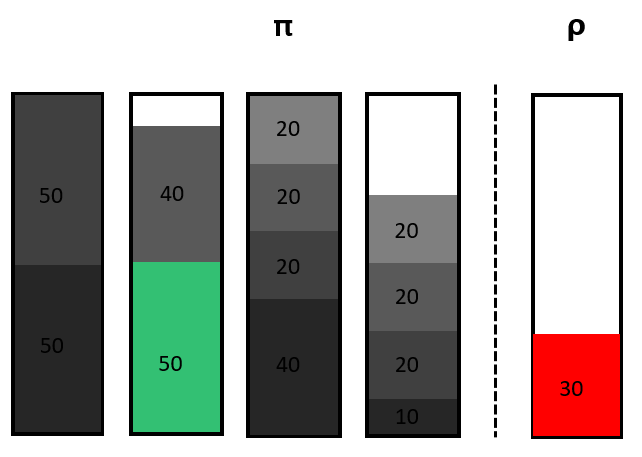
\includegraphics[scale=0.35]{img/HC_2.png}
\end{center}
\end{figure}


\end{frame}
%%%------------------------------------------------
\begin{frame}
\frametitle{4. Zusammenfügen der Gruppen}
\begin{figure}[!htbp]
\begin{center}
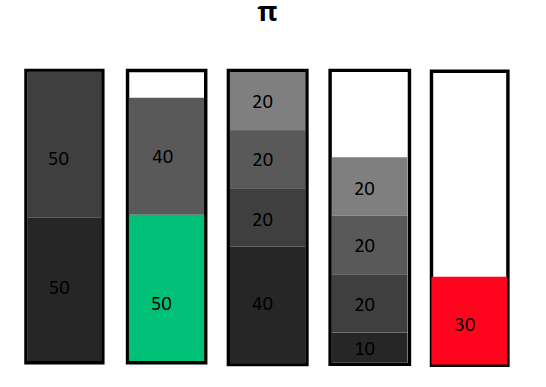
\includegraphics[scale=0.25]{img/HC_4.png}
\end{center}
\end{figure}


\end{frame}
%%%------------------------------------------------
\begin{frame}
\frametitle{5. Shuffle der Gruppen}
\begin{footnotesize}
\begin{itemize}
\item \textbf{Standardverfahren:} 5:5:3 (\textbf{Largest First}, Reverse, Random)
\end{itemize}
\end{footnotesize}
\begin{figure}[!htbp]
\begin{center}
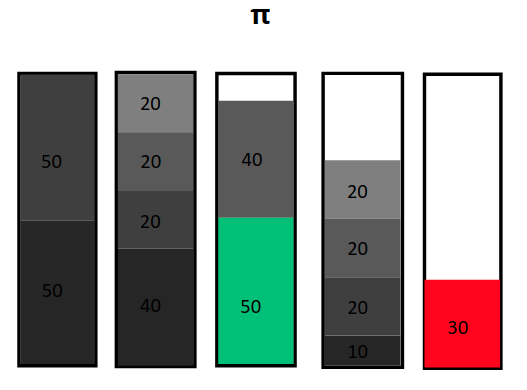
\includegraphics[scale=0.25]{img/HC_5.png}
\end{center}
\end{figure}
\begin{footnotesize}
\begin{itemize}
\item \textbf{Modifikation 1:} mittlere Itemkapazität (absteigend)
\item \textbf{Modifikation 2:} inkl. mittlere Itemkapazität (absteigend)
\item[] 5:5:5:3 (Largest First, Reverse, mittlere Itemkapazität, Random) 
\end{itemize}
\end{footnotesize}

\end{frame}
%%%------------------------------------------------
\begin{frame}
\frametitle{6. Greedy Algorithmus}
\begin{footnotesize}
\begin{itemize}
\item Ausgangslösung: $\vert U \vert = 5$ 
\item Lösung nach Greedy: $\vert U' \vert = 4$ 
\item \textbf{Theorem 1:} $\vert U'\vert \leq \vert U \vert$
\end{itemize}
\end{footnotesize}
\begin{figure}[!htbp]
\begin{center}
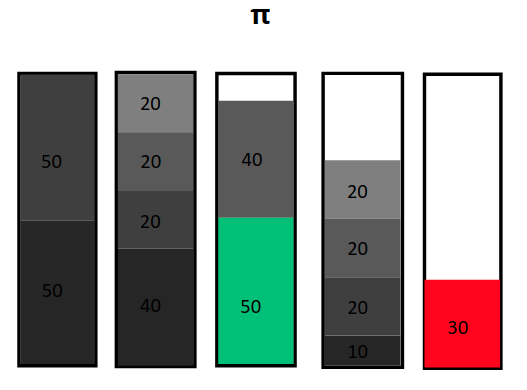
\includegraphics[scale=0.21]{img/HC_5.png}
\end{center}
\end{figure}
\begin{figure}[!htbp]
\begin{center}
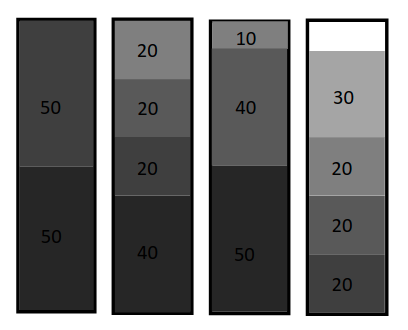
\includegraphics[scale=0.21]{img/HC_6.png}
\end{center}
\end{figure}


\end{frame}
%%%------------------------------------------------
\begin{frame}
\frametitle{Ablauf Hill Climbing Verfahren}
\begin{footnotesize}
\begin{enumerate}
\item Eröffnungsverfahren (First Fit Descending)
\item Zufällige Auswahl von Bins 
\item Ausführung des Verbesserungsverfahrens
\item Füge Gruppen wieder zusammen
\item Shuffle der Gruppen
\item Greedy Algorithmus
\item \textbf{Wiederhole Schritt 2-6 bis Abbruchkriterium erreicht}
\end{enumerate}
\end{footnotesize}
\end{frame}
%%%------------------------------------------------
%%%------------------------------------------------
%\begin{frame}
%\frametitle{3. Verbesserungsverfahren im Detail}
%\begin{figure}[!htbp]
%\begin{center}
%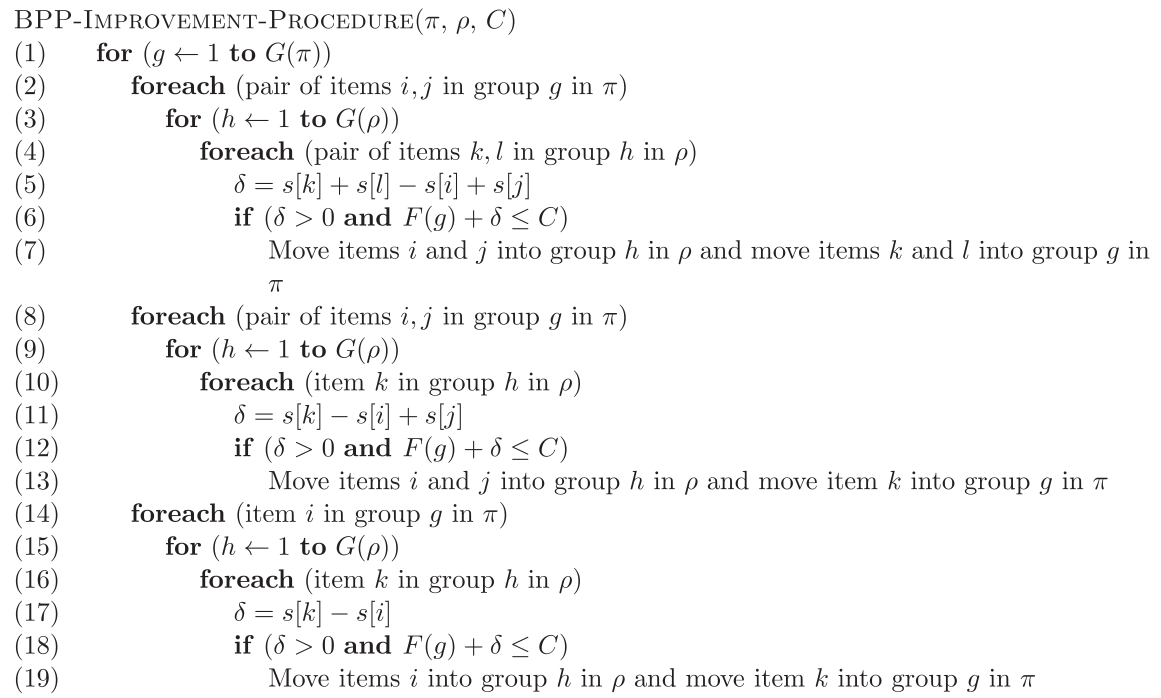
\includegraphics[scale=0.25]{img/improvement.png}
%\end{center}
%\caption{Verbesserungsverfahren Pseudocode}
%\label{fig:architecture}
%\end{figure}
%
%\end{frame}


%%%%------------------------------------------------
\begin{frame}
\frametitle{3. Verbesserungsverfahren im Detail}
\begin{algorithm}[H]
\begin{algorithmic}[1]
\begin{scriptsize}
\STATE BPP-IMPROVEMENT-PROCEDURE$(\pi,\rho,C)$
\FOR{($g=1$ to $G(\pi)$)}
\FOR{\textbf{each} (pair of items $i,j$ in group $g$ in $\pi$)}
\FOR{($h=1$ to $G(\rho)$)}
\FOR{\textbf{each} (pair of items $k,l$ in group $h$ in $\rho$)}
\STATE $\delta = s[k] + s[l] - s[i] - s[j]$
\IF{($\delta > 0$ and $F(g)+ \delta \leq C)$}
\STATE Move items $i$ and $j$ into group $h$ in $\rho$ and move items $k$ and $l$ into group $g$ in $\pi$
\ENDIF
\ENDFOR
\ENDFOR
\ENDFOR
\FOR{\textbf{each} (pair of items $i,j$ in group $g$ in $\pi$)}
\FOR{($h=1$ to $G(\rho)$)}
\FOR{\textbf{each} (item $k$ in group $h$ in $\rho$)}
\STATE $\delta = s[k] - s[i] - s[j]$
\IF{($\delta > 0$ and $F(g)+ \delta \leq C)$}
\STATE Move items $i$ and $j$ into group $h$ in $\rho$ and move items $k$ into group $g$ in $\pi$
\ENDIF
\ENDFOR
\ENDFOR
\ENDFOR
\FOR{\textbf{each} (item $i$ in group $g$ in $\pi$)}
\FOR{($h=1$ to $G(\rho)$)}
\FOR{\textbf{each} (item $k$ in group $h$ in $\rho$)}
\STATE $\delta = s[k] - s[i]$
\IF{($\delta > 0$ and $F(g)+ \delta \leq C)$}
\STATE Move items $i$  into group $h$ in $\rho$ and move item $k$ into group $g$ in $\pi$
\ENDIF
\ENDFOR
\ENDFOR
\ENDFOR
\ENDFOR
\end{scriptsize}
\end{algorithmic}
\end{algorithm}
\end{frame}

%%%------------------------------------------------
\begin{frame}
\frametitle{2:2 Move}
\begin{columns}[c] % The "c" option specifies centered vertical alignment while the "t" option is used for top vertical alignment
\column{.5\textwidth}
\begin{footnotesize}
\begin{itemize}
\item $\delta = s[k]+s[l]-s[i]-s[j]$
\item $\delta = 50 + 25 - 50 - 20 = 5$
\item $if(\delta > 0 \ and \ F(g)+\delta \leq C)$
\item $if(5 > 0 \ and \ 95+5 \leq 100)$
\end{itemize}
\end{footnotesize}
\column{.5\textwidth}
\begin{figure}[!htbp]
\begin{center}
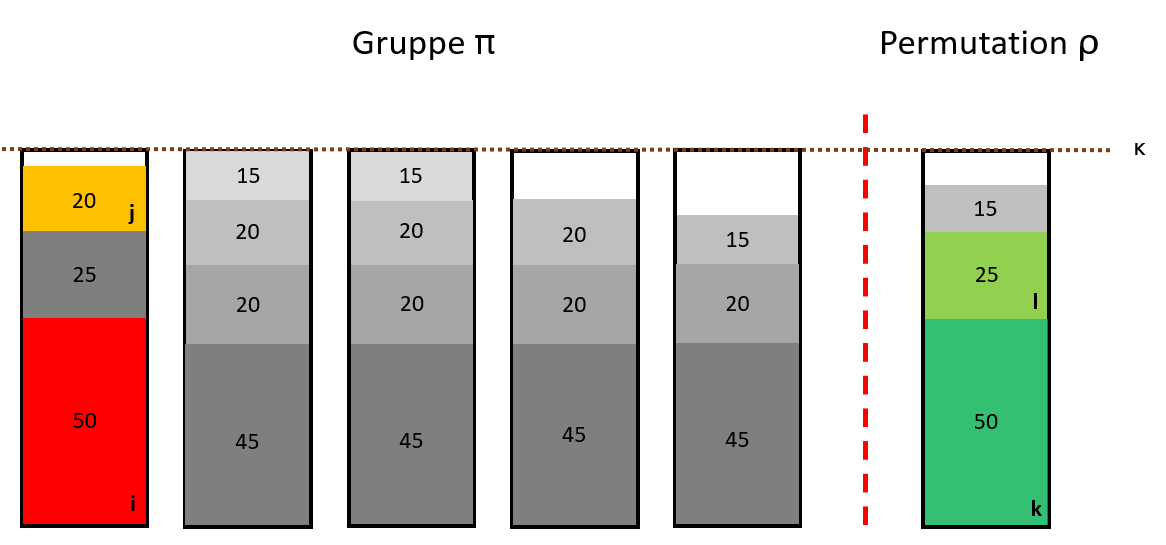
\includegraphics[scale=0.22]{img/Zwei_zwei_Move_1.png}
\end{center}
\label{fig:architecture}
\end{figure}
\begin{figure}[!htbp]
\begin{center}
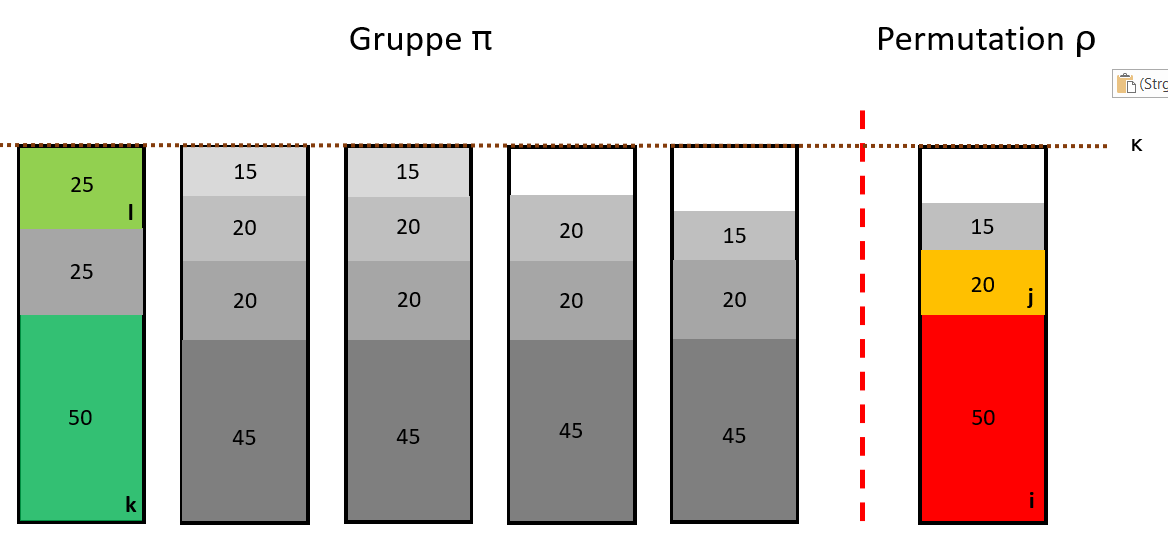
\includegraphics[scale=0.22]{img/Zwei_zwei_Move_2.png}
\end{center}
\label{fig:architecture}
\end{figure}
\end{columns}



\end{frame}
%%%------------------------------------------------
%%%------------------------------------------------
%\begin{frame}
%\frametitle{2:1 Move}
%\begin{footnotesize}
%\begin{itemize}
%\item $\delta = s[k]-s[i]-s[j]$
%\item $\delta = 45 - 20 - 20 = 5$
%\item $if(\delta > 0 \ and \ F(g)+\delta \leq C)$
%\item $if(5 > 0 \ and \ 85+5 \leq 91)$
%\end{itemize}
%\end{footnotesize}
%\begin{figure}[!htbp]
%\begin{center}
%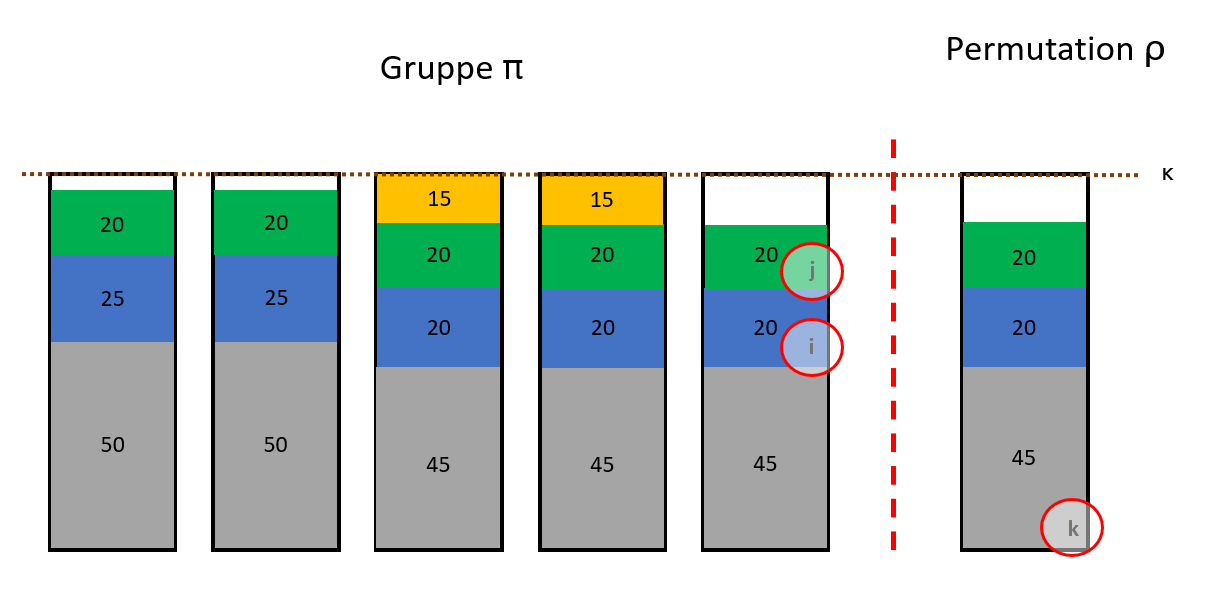
\includegraphics[scale=0.22]{img/2 zu 1 Move.png}
%\end{center}
%\label{fig:architecture}
%\end{figure}
%\begin{figure}[!htbp]
%\begin{center}
%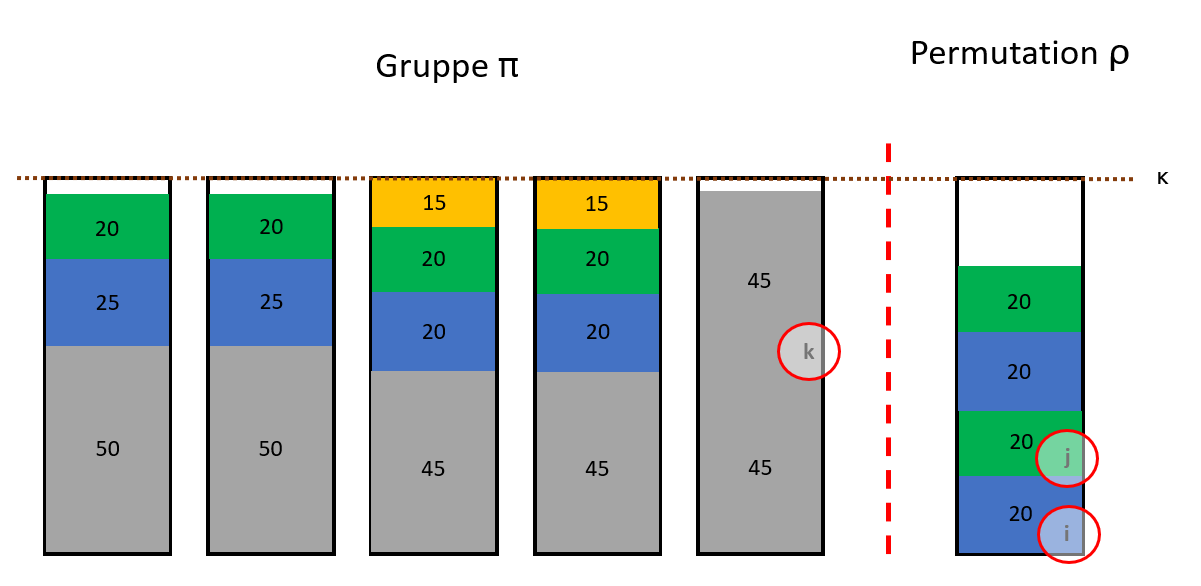
\includegraphics[scale=0.22]{img/2 zu 1 Move fertig.png}
%\end{center}
%\label{fig:architecture}
%\end{figure}
%\end{frame}
%%%------------------------------------------------
%%%------------------------------------------------
\begin{frame}
\frametitle{2:1 Move}
\begin{columns}[c] % The "c" option specifies centered vertical alignment while the "t" option is used for top vertical alignment
\column{.5\textwidth}
\begin{footnotesize}
\begin{itemize}
\item $\delta = s[k]-s[i]-s[j]$
\item $\delta = 50 - 20 - 20 = 10$
\item $if(\delta > 0 \ and \ F(g)+\delta \leq C)$
\item $if(10 > 0 \ and \ 85+10 \leq 100)$
\end{itemize}
\end{footnotesize}
\column{.5\textwidth}
\begin{figure}[!htbp]
\begin{center}
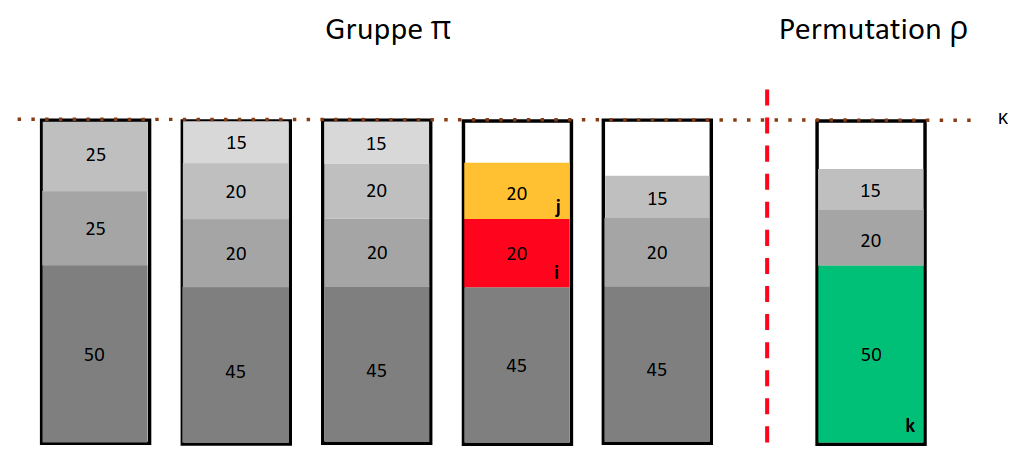
\includegraphics[scale=0.15]{img/Zwei_Eins_Move_1.png}
\end{center}
\label{fig:architecture}
\end{figure}
\begin{figure}[!htbp]
\begin{center}
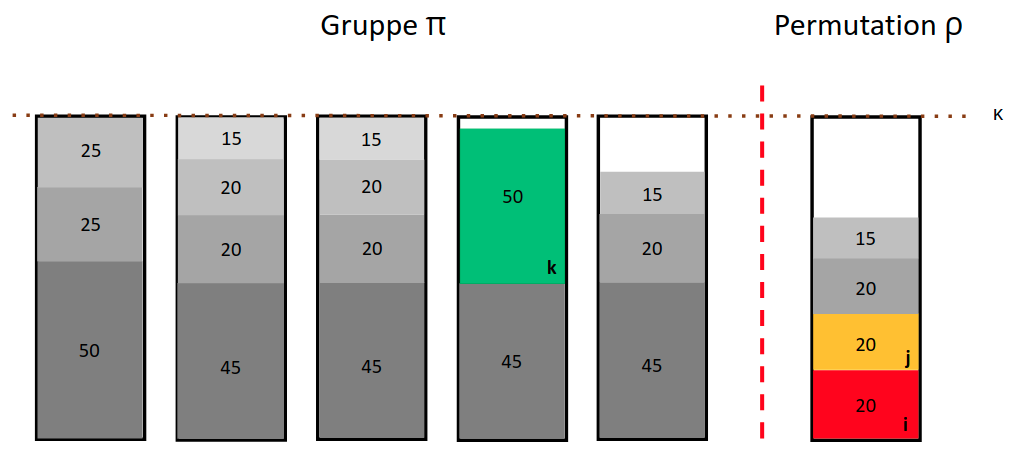
\includegraphics[scale=0.15]{img/Zwei_Eins_Move_2.png}
\end{center}
\label{fig:architecture}
\end{figure}
\end{columns}
\end{frame}
%%%------------------------------------------------
%%%------------------------------------------------
\begin{frame}
\frametitle{1:1 Move}
\begin{columns}[c] % The "c" option specifies centered vertical alignment while the "t" option is used for top vertical alignment
\column{.5\textwidth}
\begin{footnotesize}
\begin{itemize}
\item $\delta = s[k]-s[i]$
\item $\delta = 20 - 15 = 5$
\item $if(\delta > 0 \ and \ F(g)+\delta \leq C)$
\item $if(5 > 0 \ and \ 80 + 5 \leq 100)$
\end{itemize}
\end{footnotesize}
\column{.5\textwidth}
\begin{figure}[!htbp]
\begin{center}
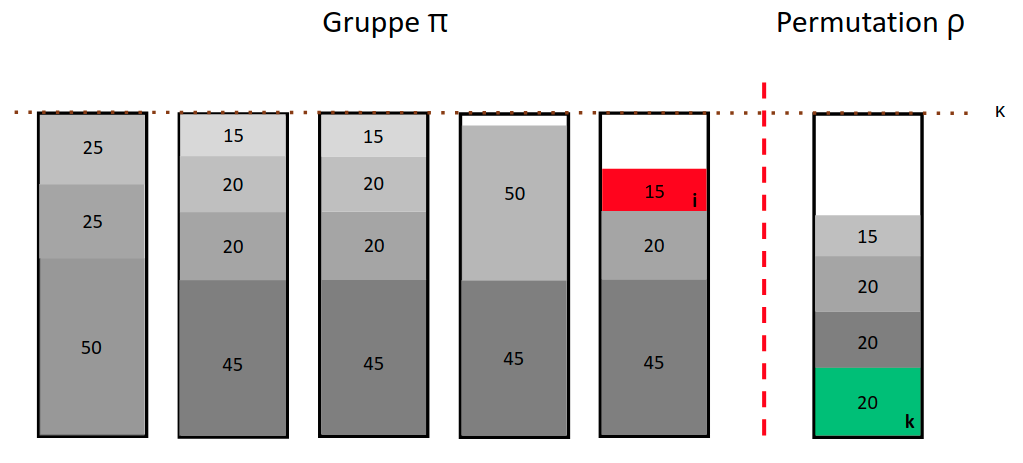
\includegraphics[scale=0.15]{img/1zu1_1.png}
\end{center}
\label{fig:architecture}
\end{figure}
\begin{figure}[!htbp]
\begin{center}
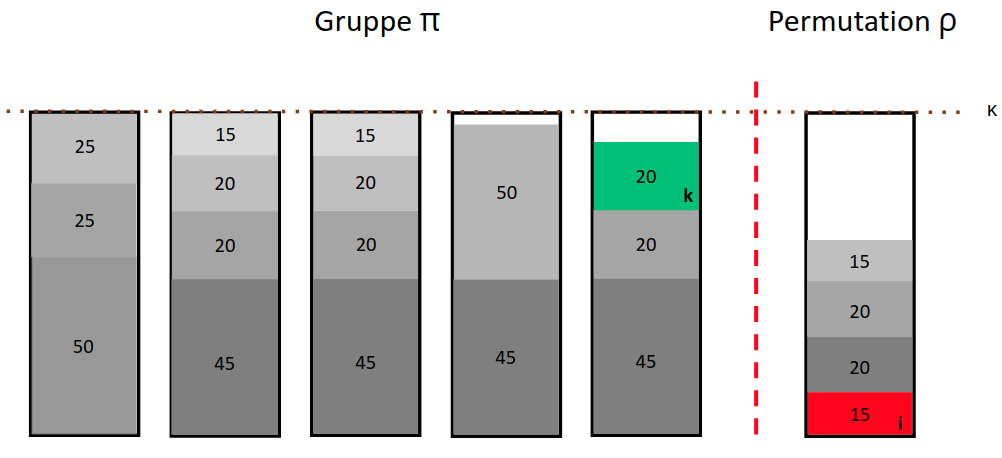
\includegraphics[scale=0.15]{img/1zu1_2.png}
\end{center}
\label{fig:architecture}
\end{figure}
\end{columns}
\end{frame}
%%%------------------------------------------------
%%%------------------------------------------------
%\begin{frame}
%\frametitle{Verbesserungsverfahren}
%\begin{figure}[!htbp]
%\begin{center}
%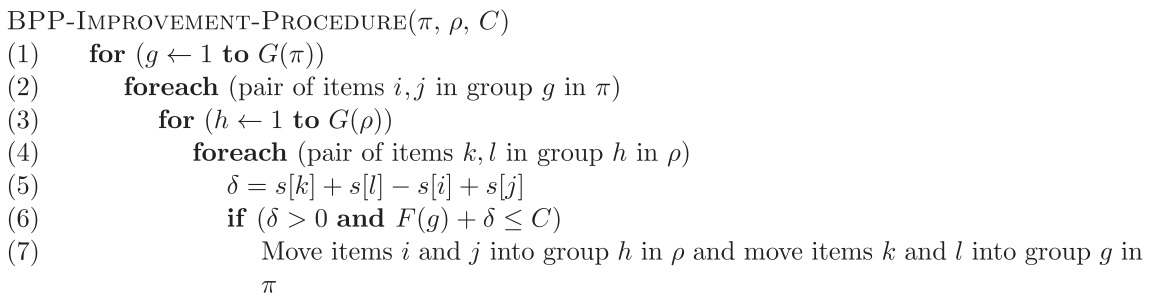
\includegraphics[scale=0.25]{img/improve1.png}
%\end{center}
%\caption{Verbesserungsverfahren Pseudocode}
%\label{fig:architecture}
%\end{figure}
%\end{frame}
%%%%------------------------------------------------
%\begin{frame}
%\frametitle{2:2 Move}
%
%\end{frame}
%%%------------------------------------------------
\section{Computational Studies}
\begin{frame}
\frametitle{Computational Studies - Set-up}

\begin{table}
\begin{footnotesize}
\begin{tabular}{c c c c c c}
\toprule
\textbf{Typ} & \textbf{\#Instanzen} & \textbf{\#Items} & \textbf{Bin-Kapazität} & \textbf{Verteilung} & \textbf{Notation}\\
\midrule
Uniform  & 20   & 120 & 150 & 20-100 & (U,120,150) \\
Uniform  & 20   & 250 & 150 & 20-100 & (U,250,150) \\
Uniform  & 20   & 500 & 150 & 20-100 & (U,500,150) \\
Uniform  & 20   & 1000 & 150 & 20-100 & (U,1000,150) \\\midrule
Hard  & 10   & 200 & 100000 & 20000-35000 & (H,200,100000) \\\midrule
Triplet  & 20   & 60 & 1000 & * & (T,60,1000) \\
Triplet  & 20   & 120 & 1000 & * & (T,120,1000) \\
Triplet  & 20   & 249 & 1000 & * & (T,249,1000) \\
Triplet  & 20   & 501 & 1000 & * & (T,501,1000) \\
\bottomrule
\end{tabular}
\end{footnotesize}
%\caption{Ergebnisse}
\end{table}
\begin{footnotesize}
\begin{itemize}
\item * optimale Lösung hat 3 Items pro Bin (ein großes Item und zwei kleine Items)
\item Python 3.8.5
\item Intel Core i7-7Y75, 8GB RAM
\item SEED = 123
\end{itemize}
\end{footnotesize}

\end{frame}
%%%------------------------------------------------
%\begin{frame}
%\frametitle{Verbesserungsverfahren}
%\begin{figure}[!htbp]
%\begin{center}
%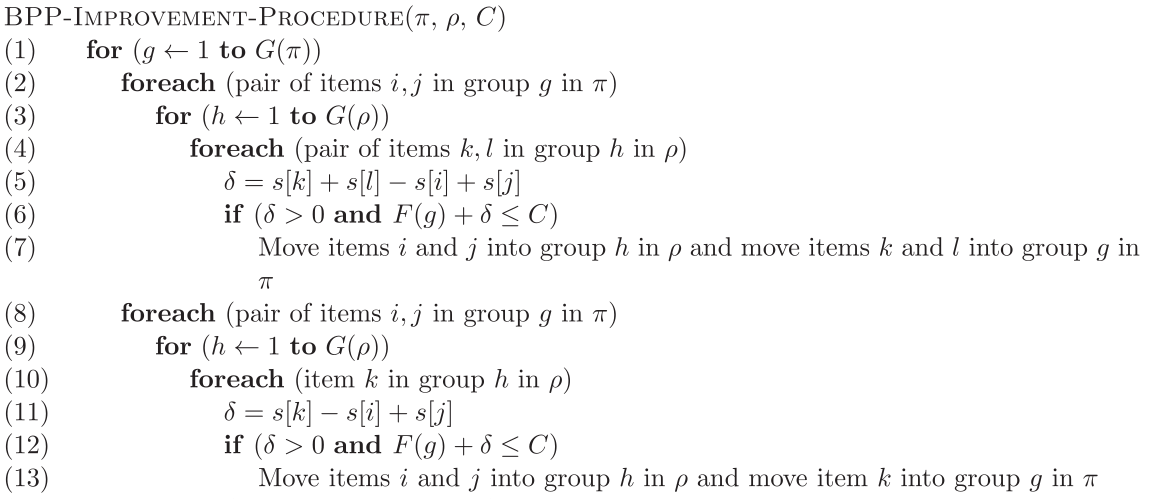
\includegraphics[scale=0.25]{img/improve2.png}
%\end{center}
%\caption{Verbesserungsverfahren Pseudocode}
%\label{fig:architecture}
%\end{figure}
%\end{frame}
%%%%------------------------------------------------
%\begin{frame}
%\frametitle{2:1 Move}
%
%\end{frame}
%%%%------------------------------------------------
%%%%------------------------------------------------
%\begin{frame}
%\frametitle{Verbesserungsverfahren}
%\begin{figure}[!htbp]
%\begin{center}
%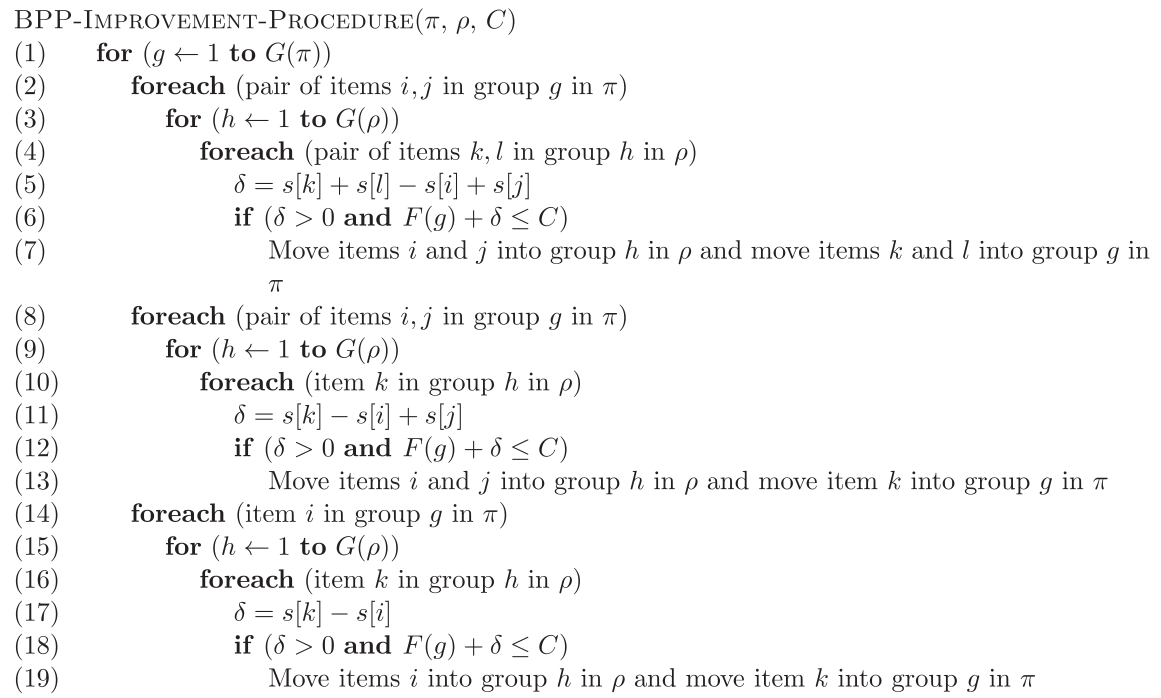
\includegraphics[scale=0.25]{img/improvement.png}
%\end{center}
%\caption{Verbesserungsverfahren Pseudocode}
%\label{fig:architecture}
%\end{figure}
%
%\end{frame}
%%%%------------------------------------------------
%\begin{frame}
%\frametitle{1:1 Move}
%
%\end{frame}
%%%------------------------------------------------
%----------------------------------------------------------------------------------------
\begin{frame}
\frametitle{Übersicht der Ergebnisse}
\begin{footnotesize}
\begin{itemize}
\item $LB = \left\lceil\sum_{j=1}^{n} \frac{w_j}{C}\right\rceil$
\item \textbf{Uniform}: $LB = z^{*}$ bei \textbf{79 von 80 Instanzen} (eine Instanz mit $z^{*} = LB + 1$)
\item \textbf{Hard}: $LB = z^{*}$ bei \textbf{3 von 10 Instanzen} (Bei 7 von 10 $z^{*} = LB + 1$) 
\item \textbf{Triplet}: $LB = z^{*}$ für \textbf{alle Instanzen} 
\end{itemize}
\end{footnotesize}

\begin{scriptsize}
\begin{table}
\begin{tabular}{l c c c c c c c}
\toprule
\textbf{Typ} & \textbf{Inst.} &  \textbf{Mittlere LB} & \textbf{FFD} & \textbf{HC} & \textbf{HC*}  & \textbf{Mittlere Zeit}\\
\midrule
(U,120,150)  & 20    & 49.1  & 0.7 & \textbf{0.05} & \textbf{0.1} & 6.24 \\
(U,250,150)  & 20     & 101.6  & 1.5 & \textbf{0.25} & \textbf{0.25} & 27.19 \\
(U,500,150)  & 20     & 201.2  & 2.7 & \textbf{0.15} & \textbf{0.15} &  25.73\\
(U,1000,150)  & 20     & 400.6  & 4.85 & \textbf{0.25} & \textbf{0.2} & 42.91\\ \midrule
(H,200,100000)  & 10     & 55.5/56.2  & 4.1/3.4 & \textbf{0.8} &\textbf{0} & 81.04 \\\midrule
(T,60,1000)  & 20      & 20  & 3.2 & \textbf{1} &\textbf{0.85} & 100 \\
(T,120,1000)  & 20     & 40  & 5.8 & \textbf{1} &\textbf{1} & 100 \\
(T,249,1000)  & 20     & 83  & 12.1 & \textbf{1} &\textbf{1} & 100 \\
(T,501,1000)  & 20     & 167  & 23.05 & \textbf{1.1} &\textbf{1} & 100 \\
\bottomrule
\end{tabular}
%\caption{Ergebnisse}
\end{table}
\end{scriptsize}

\end{frame}


%----------------------------------------------------------------------------------------




\begin{frame}

\frametitle{Optimalitätsanalyse Instanzgruppe Uniform \& Hard}
\begin{footnotesize}
\begin{itemize}
\item Uniform \textbf{20 Instanzen} pro Gruppe und Hard \textbf{10 Instanzen}
\item $LB = \left\lceil\sum_{j=1}^{n} \frac{w_j}{C}\right\rceil$
\end{itemize}
\end{footnotesize}


\begin{figure}[!htbp]
\begin{center}
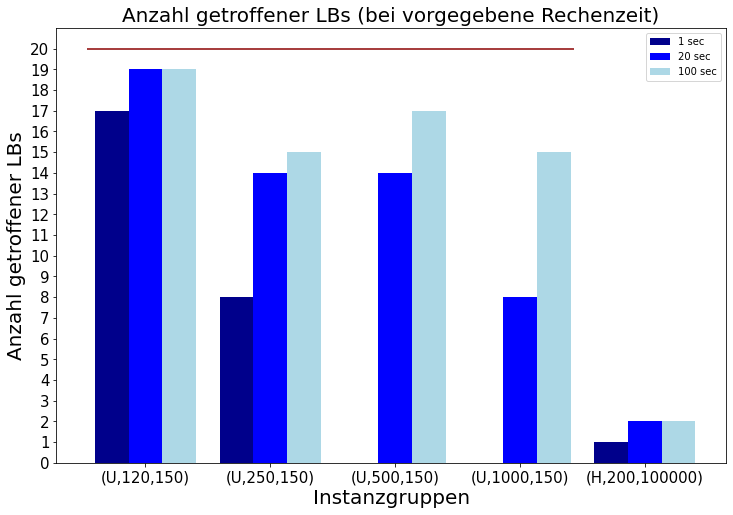
\includegraphics[scale=0.3]{img/lb_unif_hard.png}
\end{center}
\caption{Anzahl getroffener LBs}
\label{fig:LBs}
\end{figure}



\end{frame}
%----------------------------------------------------------------------------------------
\begin{frame}

\frametitle{Worst Case Analyse Instanzgruppe Uniform \& Hard}
\begin{footnotesize}
\begin{itemize}
\item Uniform \textbf{20 Instanzen} pro Gruppe und Hard \textbf{10 Instanzen}
\item $LB = \left\lceil\sum_{j=1}^{n} \frac{w_j}{C}\right\rceil$
\end{itemize}
\end{footnotesize}
\begin{figure}[!htbp]
\begin{center}
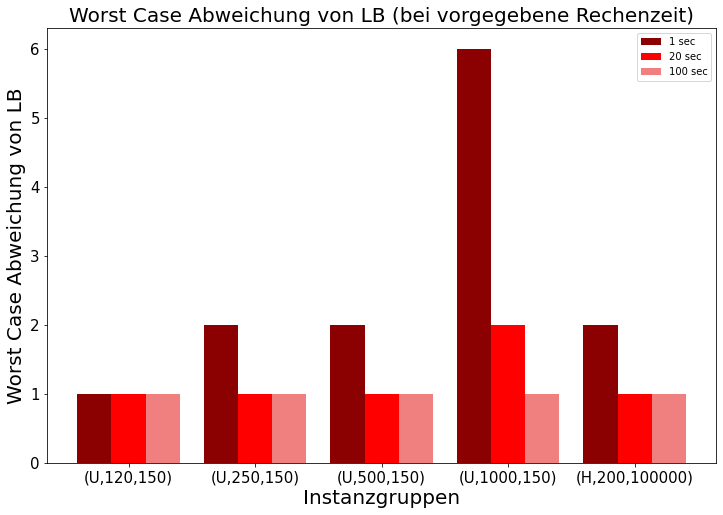
\includegraphics[scale=0.3]{img/wc_unif_hard.png}
\end{center}
\caption{Worst Case Abweichung von LB}
\label{fig:WC}
\end{figure}



\end{frame}
%----------------------------------------------------------------------------------------
\begin{frame}

\frametitle{Lösungsgüte im Zeitverlauf Instanzgruppe Uniform \& Hard }

\begin{figure}[!htbp]
\begin{center}
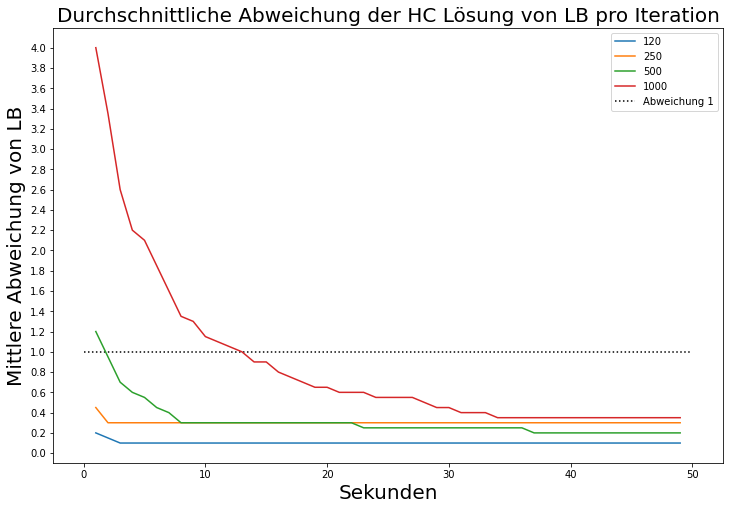
\includegraphics[scale=0.35]{img/uniform_time.png}
\end{center}
\caption{Mittlere Abweichung von LB pro Zeiteinheit}
\label{fig:architecture}
\end{figure}

\end{frame}

%----------------------------------------------------------------------------------------
\begin{frame}

\frametitle{Optimalitätsanalyse Instanzgruppe Triplet}
\begin{footnotesize}
\begin{itemize}
\item $LB = \left\lceil\sum_{j=1}^{n} \frac{w_j}{C}\right\rceil = \frac{\#Items}{3} $
\item LB wird nie getroffen
\end{itemize}

\end{footnotesize}


\begin{figure}[!htbp]
\begin{center}
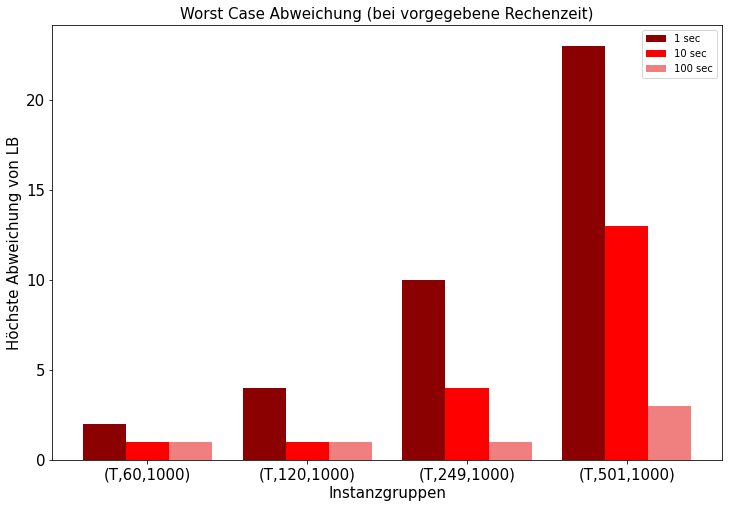
\includegraphics[scale=0.3]{img/wc_trip.png}
\end{center}
\caption{Worst Case Abweichung von LB}
\label{fig:architecture}
\end{figure}



\end{frame}
%----------------------------------------------------------------------------------------
\begin{frame}

\frametitle{Lösungsgüte im Zeitverlauf Instanzgruppe Triplet}

\begin{figure}[!htbp]
\begin{center}
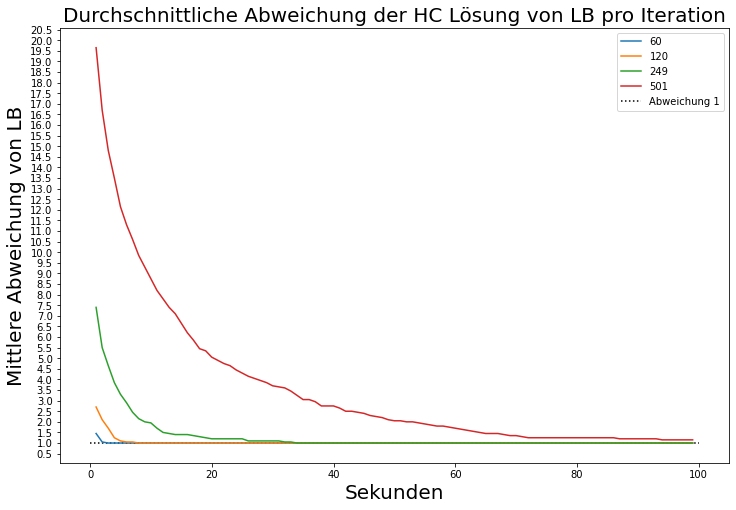
\includegraphics[scale=0.3]{img/triplet_time.png}
\end{center}
\caption{Mittlere Abweichung von LB pro Zeiteinheit}
\label{fig:architecture}
\end{figure}

\end{frame}
%----------------------------------------------------------------------------------------
\begin{frame}
\frametitle{Vergleich Uniform, Hard und Triplet}


\begin{columns}[c] % The "c" option specifies centered vertical alignment while the "t" option is used for top vertical alignment

\column{.5\textwidth} % Left column and width
\begin{figure}[!htbp]
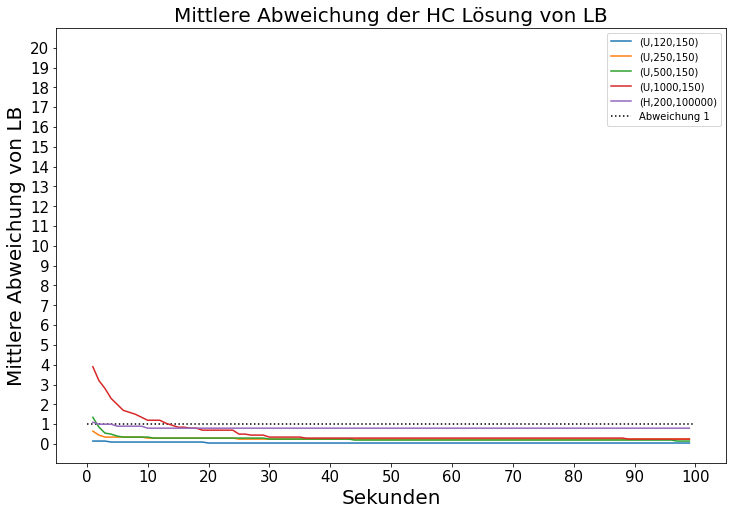
\includegraphics[scale=0.2]{img/unif_hard_time_vergleich.png}
\caption{Uniform und Hard}
\label{fig:architecture}
\end{figure}


\column{.5\textwidth} % Right column and width
\begin{figure}[!htbp]
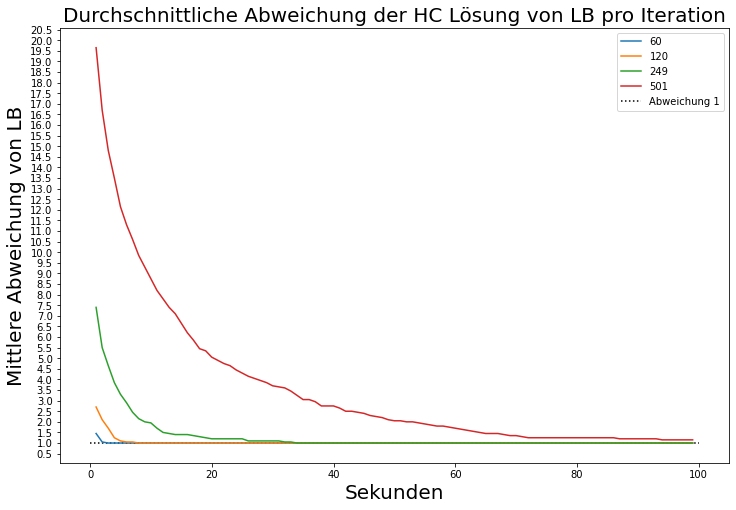
\includegraphics[scale=0.2]{img/triplet_time.png}
\caption{Triplet}
\label{fig:architecture}
\end{figure}


\end{columns}
\end{frame}

%----------------------------------------------------------------------------------------
%----------------------------------------------------------------------------------------
%----------------------------------------------------------------------------------------
\begin{frame}

\frametitle{Verteilungsfunktion}

\begin{footnotesize}
\begin{equation}
mit \ r = \frac{Z_{HC}-LB}{LB} * 100\%
\end{equation}
\end{footnotesize}

\begin{figure}[!htbp]
\begin{center}
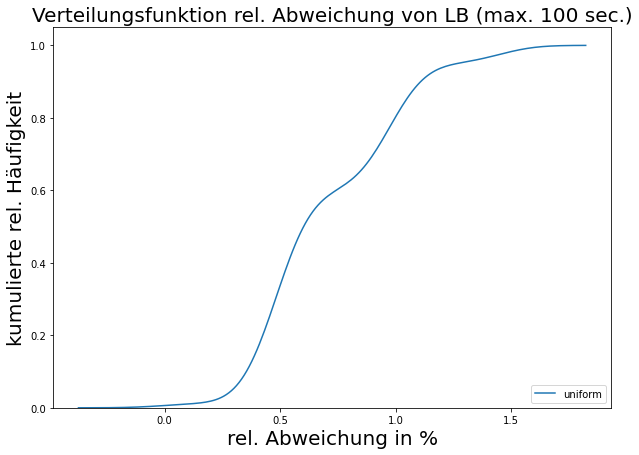
\includegraphics[scale=0.3]{img/dist1.png}
\end{center}
\caption{rel. Abweichung von LB}
\label{fig:architecture}
\end{figure}



\end{frame}
%----------------------------------------------------------------------------------------
%----------------------------------------------------------------------------------------
\begin{frame}

\frametitle{Verteilungsfunktion}

\begin{footnotesize}
\begin{equation}
mit \ r = \frac{Z_{HC}-LB}{LB} * 100\%
\end{equation}
\end{footnotesize}

\begin{figure}[!htbp]
\begin{center}
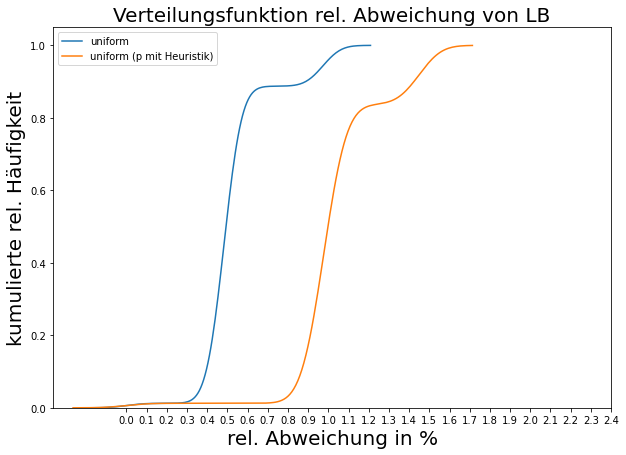
\includegraphics[scale=0.3]{img/dist2.png}
\end{center}
\caption{rel. Abweichung von LB}
\label{fig:architecture}
\end{figure}



\end{frame}
%----------------------------------------------------------------------------------------
%----------------------------------------------------------------------------------------
\begin{frame}

\frametitle{Verteilungsfunktion}

\begin{footnotesize}
\begin{equation}
mit \ r = \frac{Z_{HC}-LB}{LB} * 100\%
\end{equation}
\end{footnotesize}

\begin{figure}[!htbp]
\begin{center}
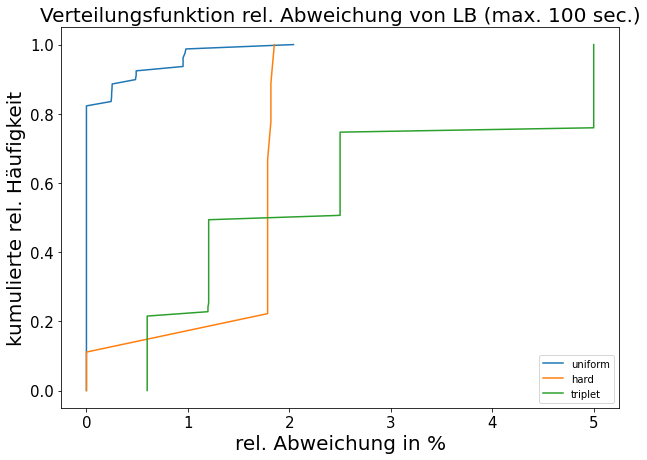
\includegraphics[scale=0.3]{img/dist3.png}
\end{center}
\caption{rel. Abweichung von LB}
\label{fig:architecture}
\end{figure}



\end{frame}
%----------------------------------------------------------------------------------------

%----------------------------------------------------------------------------------------
\begin{frame}

\frametitle{Verteilungsfunktion - Verfahrensänderung (Uniform)}

\begin{footnotesize}
\begin{equation}
mit \ r = \frac{Z_{HC}-LB}{LB} * 100\%
\end{equation}
\end{footnotesize}

\begin{figure}[!htbp]
\begin{center}
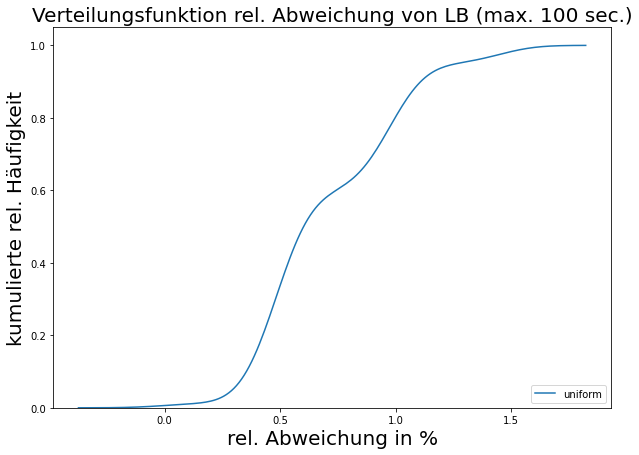
\includegraphics[scale=0.3]{img/dist1.png}
\end{center}
\caption{rel. Abweichung von LB}
\label{fig:architecture}
\end{figure}



\end{frame}
%----------------------------------------------------------------------------------------
%----------------------------------------------------------------------------------------
\begin{frame}

\frametitle{Verteilungsfunktion - andere Permutationswahl}

\begin{footnotesize}
\begin{equation}
mit \ r = \frac{Z_{HC}-LB}{LB} * 100\%
\end{equation}
\end{footnotesize}

\begin{figure}[!htbp]
\begin{center}
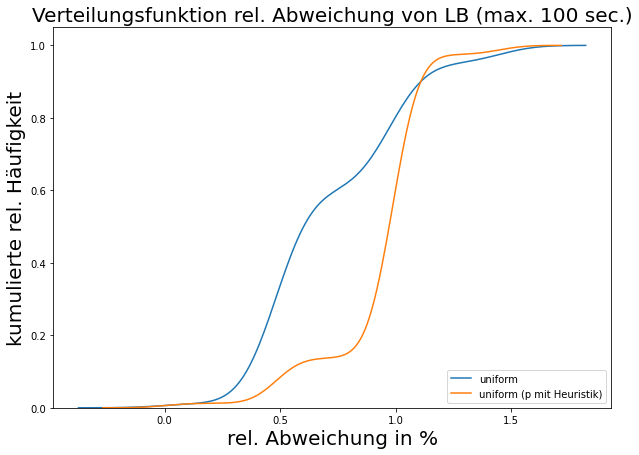
\includegraphics[scale=0.3]{img/dist4.png}
\end{center}
\caption{rel. Abweichung von LB}
\label{fig:architecture}
\end{figure}



\end{frame}
%----------------------------------------------------------------------------------------
%----------------------------------------------------------------------------------------
\begin{frame}

\frametitle{Verteilungsfunktion - Shuffle (mittlere Itemkapazität)}

\begin{footnotesize}
\begin{equation}
mit \ r = \frac{Z_{HC}-LB}{LB} * 100\%
\end{equation}
\end{footnotesize}

\begin{figure}[!htbp]
\begin{center}
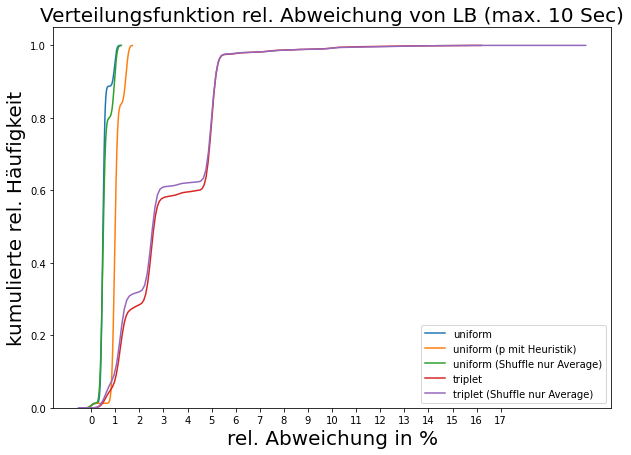
\includegraphics[scale=0.3]{img/dist5.png}
\end{center}
\caption{rel. Abweichung von LB}
\label{fig:architecture}
\end{figure}



\end{frame}
%----------------------------------------------------------------------------------------
%----------------------------------------------------------------------------------------
\begin{frame}

\frametitle{Verteilungsfunktion - Shuffle (inkl. mittlere Itemkapazität)}

\begin{footnotesize}
\begin{equation}
mit \ r = \frac{Z_{HC}-LB}{LB} * 100\%
\end{equation}
\end{footnotesize}

\begin{figure}[!htbp]
\begin{center}
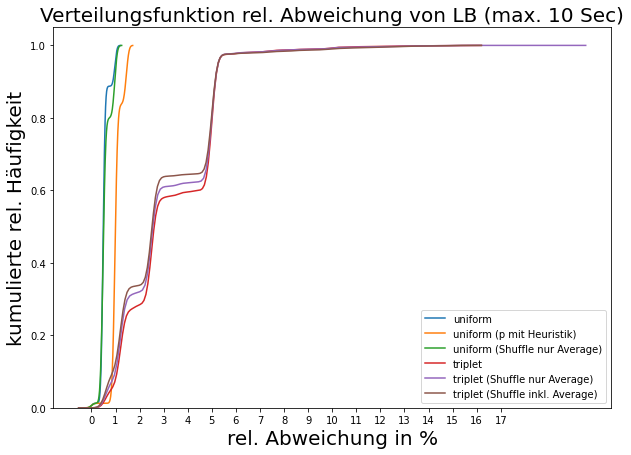
\includegraphics[scale=0.3]{img/dist6.png}
\end{center}
\caption{rel. Abweichung von LB}
\label{fig:architecture}
\end{figure}



\end{frame}
%----------------------------------------------------------------------------------------

%----------------------------------------------------------------------------------------

%----------------------------------------------------------------------------------------
\begin{frame}

\frametitle{Verteilungsfunktion - Verfahrensänderung (Triplet)}

\begin{footnotesize}
\begin{equation}
mit \ r = \frac{Z_{HC}-LB}{LB} * 100\%
\end{equation}
\end{footnotesize}

\begin{figure}[!htbp]
\begin{center}
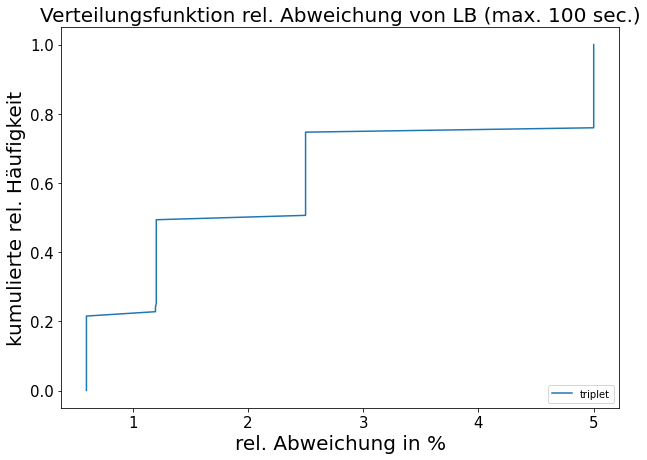
\includegraphics[scale=0.3]{img/dist7.png}
\end{center}
\caption{rel. Abweichung von LB}
\label{fig:architecture}
\end{figure}



\end{frame}
%----------------------------------------------------------------------------------------
%----------------------------------------------------------------------------------------
%\begin{frame}
%
%\frametitle{Verteilungsfunktion - Shuffle (mittlere Itemkapazität)}
%
%\begin{footnotesize}
%\begin{equation}
%mit \ r = \frac{Z_{HC}-LB}{LB} * 100\%
%\end{equation}
%\end{footnotesize}
%
%\begin{figure}[!htbp]
%\begin{center}
%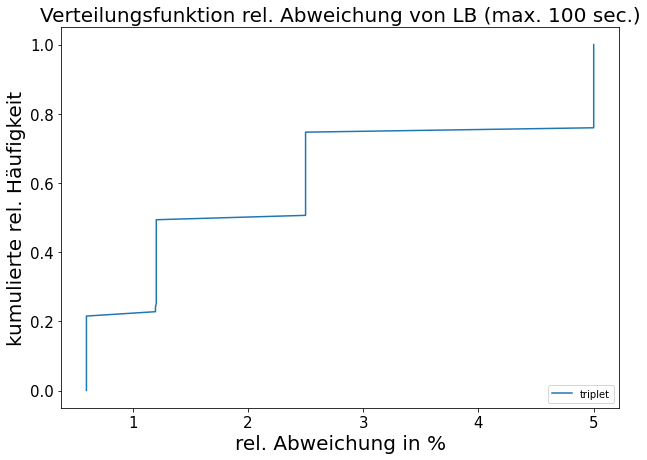
\includegraphics[scale=0.3]{img/dist7.png}
%\end{center}
%\caption{rel. Abweichung von LB}
%\label{fig:architecture}
%\end{figure}
%
%
%
%\end{frame}
%----------------------------------------------------------------------------------------
%----------------------------------------------------------------------------------------
\begin{frame}

\frametitle{Verteilungsfunktion - Shuffle (mittlere Itemkapazität)}

\begin{footnotesize}
\begin{equation}
mit \ r = \frac{Z_{HC}-LB}{LB} * 100\%
\end{equation}
\end{footnotesize}

\begin{figure}[!htbp]
\begin{center}
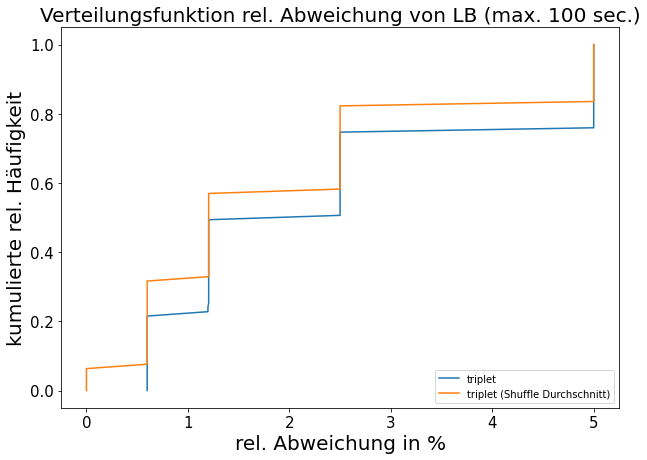
\includegraphics[scale=0.3]{img/dist8.png}
\end{center}
\caption{rel. Abweichung von LB}
\label{fig:architecture}
\end{figure}



\end{frame}
%----------------------------------------------------------------------------------------
%----------------------------------------------------------------------------------------
\begin{frame}

\frametitle{Verteilungsfunktion - Shuffle (inkl. mittlere Itemkapazität)}

\begin{footnotesize}
\begin{equation}
mit \ r = \frac{Z_{HC}-LB}{LB} * 100\%
\end{equation}
\end{footnotesize}

\begin{figure}[!htbp]
\begin{center}
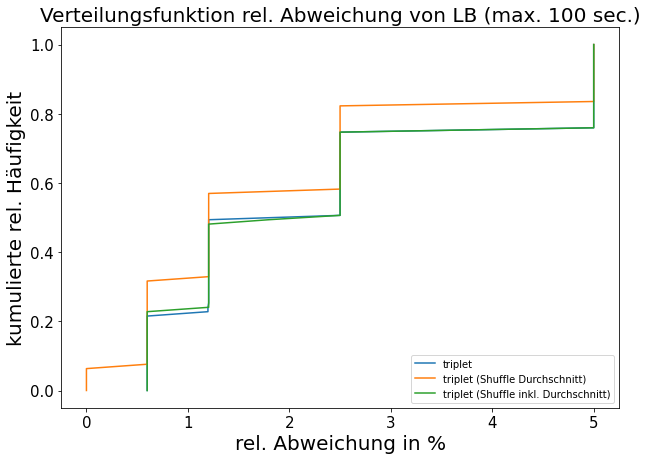
\includegraphics[scale=0.3]{img/dist9.png}
\end{center}
\caption{rel. Abweichung von LB}
\label{fig:architecture}
\end{figure}



\end{frame}
%----------------------------------------------------------------------------------------

%----------------------------------------------------------------
\section{Zusammenfassung} 
\begin{frame}
\frametitle{Zusammenfassung und Ausblick}
\begin{itemize}
\item HC-Ansatz zur Lösung des Bin Packing Problems
\begin{itemize}
\item Eröffnungsheuristik: FFD
\item Verbesserunsgverfahren mit First Fit Ansatz
\end{itemize}
\item[] 
\item Ausblick Computational Studies
\begin{itemize}
\item Weitere Untersuchungen des Shuffle-Operators
\item Weglassen von Moves
\end{itemize}
\end{itemize}


\end{frame}
%----------------------------------------------------------------------------------------
\begin{frame}
\frametitle{Vergleich der Ergebnisse mit weiteren Verfahren}

\begin{scriptsize}
\begin{table}
\begin{tabular}{c c c c c c c c}
\toprule
\textbf{Typ} &   \textbf{Mittlere LB} & \textbf{FFD} & \textbf{HC} & \textbf{HC*}  & \textbf{IG$^1$} & \textbf{HGGA$^2$} & \textbf{MT$^3$}\\
\midrule
(U,120,150) & 49.1  & 0.7 & 0.05 & 0.1 & 0.7 & 0 & 0.05 \\
(U,250,150) & 101.6  & 1.5 & 0.25 & 0.25 & 1.45 & 0 & 0.55\\
(U,500,150)  & 201.2  & 2.7 & 0.15 & 0.15 &  2.7 & 0 & 2.2\\
(U,1000,150)  & 400.6  & 4.85 & 0.25 & 0.2 & 4.85 & 0 & 3.85\\ \midrule
(H,200,100000)  & 55.5/56.2  & 4.1/3.4 & 0.8 & 0 & 2.3 & 0.1 & 1.5 \\\midrule
(T,60,1000)     & 20 & 3.2 & 1 & 0.85 & 2.45 & 0.6 & 1.45 \\
(T,120,1000)    & 40  & 5.8 & 1 &1 & 5.3 & 0.85 & 4.1\\
(T,249,1000)      & 83  & 12.1 & 1 & 1 & 11.25 & 0 & 7.45 \\
(T,501,1000)      & 167  & 23.05 & 1.1 & 1 & 22.4 & 0 & 14.85 \\
\bottomrule
\end{tabular}
%\caption{Ergebnisse}
\end{table}
\end{scriptsize}
\begin{scriptsize}
\begin{itemize}
\item[1] Culberson J, Luo F. (1996)
\item[2] Falkenauer E. (1998)
\item[3] Martello S, Toth P. (1990)
\end{itemize}
\end{scriptsize}


\end{frame}
%----------------------------------------------------------------
%----------------------------------------------------------------------------------------
\begin{frame}
\frametitle{Vergleich der Ergebnisse mit weiteren Verfahren}

\begin{scriptsize}
\begin{table}
\begin{tabular}{c c c c c c c }
\toprule
\textbf{Typ} &   \textbf{Mittlere LB} & \textbf{FFD} & \textbf{HC} & \textbf{HC*}  & \textbf{HACO$^4$} & \textbf{BISON$^5$}\\
\midrule
(U,120,150) & 49.1  & 0.7 & 0.05 & 0.1 & 0 & -\\
(U,250,150) & 101.6  & 1.5 & 0.25 & 0.25 & 0.1 & -\\
(U,500,150)  & 201.2  & 2.7 & 0.15 & 0.15 &  0 & -\\
(U,1000,150)  & 400.6  & 4.85 & 0.25 & 0.2 & 0 & -\\ \midrule
(H,200,100000)  & 55.5/56.2  & 4.1/3.4 & 0.8 & 0 & - & 0.7 \\\midrule
(T,60,1000)     & 20 & 3.2 & 1 & 0.85 & - & - \\
(T,120,1000)    & 40  & 5.8 & 1 &1 & - & - \\
(T,249,1000)      & 83  & 12.1 & 1 & 1 & - & -\\
(T,501,1000)      & 167  & 23.05 & 1.1 & 1 & - & - \\
\bottomrule
\end{tabular}
%\caption{Ergebnisse}
\end{table}
\end{scriptsize}
\begin{scriptsize}
\begin{itemize}
\item[4] Levine J, Ducatelle F. (2003)
\item[5] Scholl A, Klein R, Jurgens C. (1997)
\end{itemize}
\end{scriptsize}

\end{frame}
%----------------------------------------------------------------
%----------------------------------------------------------------------------------------
%----------------------------------------------------------------------------------------

\begin{frame}
\frametitle{Triplet: Vergleich mit Shuffle (mittlere Itemkapazität)}


\begin{columns}[c] % The "c" option specifies centered vertical alignment while the "t" option is used for top vertical alignment

\column{.5\textwidth} % Left column and width
\begin{figure}[!htbp]
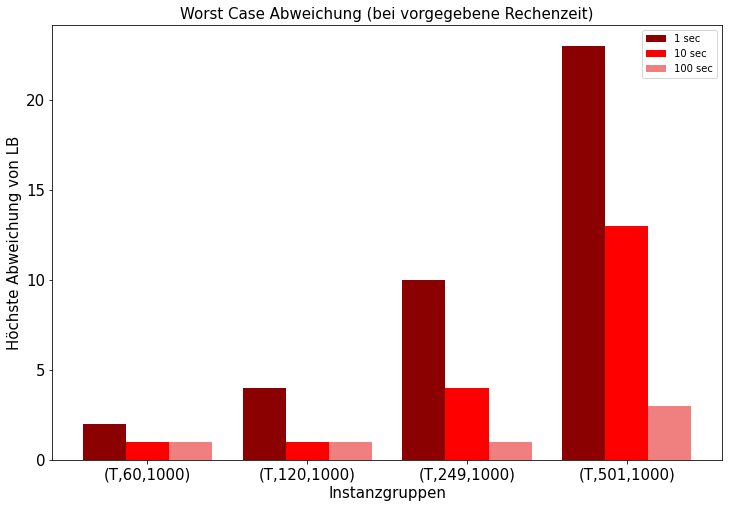
\includegraphics[scale=0.2]{img/wc_trip.png}
\caption{Standardverfahren}
\label{fig:architecture}
\end{figure}


\column{.5\textwidth} % Right column and width
\begin{figure}[!htbp]
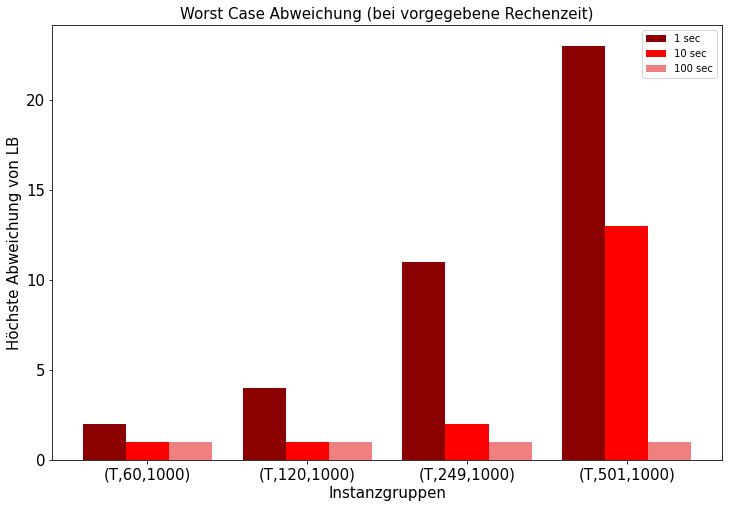
\includegraphics[scale=0.2]{img/shuffleWC.png}
\caption{mittlere Itemkapazität}
\label{fig:architecture}
\end{figure}


\end{columns}
\end{frame}
%----------------------------------------------------------------------------------------

\begin{frame}
\frametitle{Uniform: Vergleich mit anderer Permutationswahl}


\begin{columns}[c] % The "c" option specifies centered vertical alignment while the "t" option is used for top vertical alignment

\column{.5\textwidth} % Left column and width
\begin{figure}[!htbp]
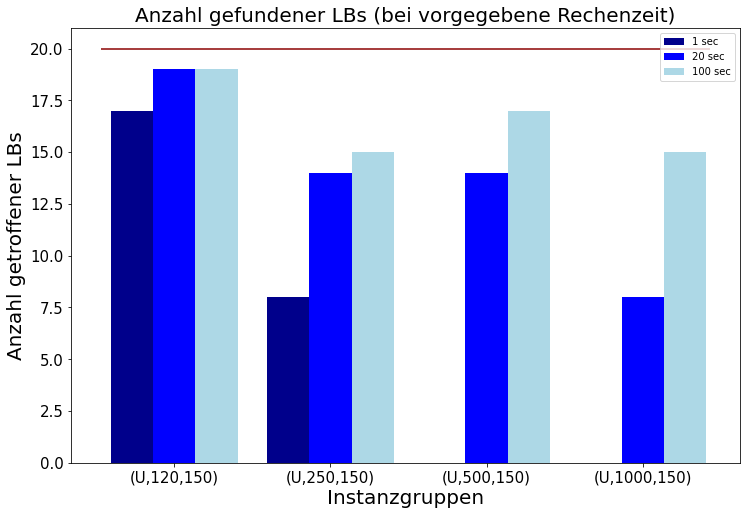
\includegraphics[scale=0.2]{img/lb_unif.png}
\caption{Random Permutation}
\label{fig:architecture}
\end{figure}


\column{.5\textwidth} % Right column and width
\begin{figure}[!htbp]
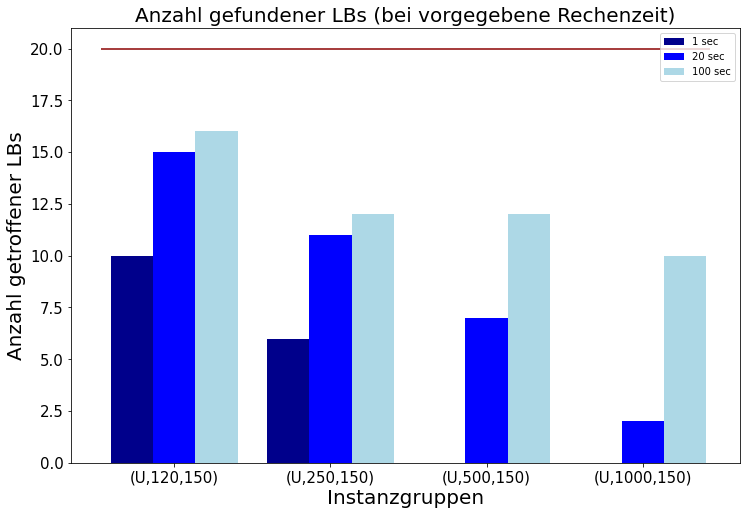
\includegraphics[scale=0.2]{img/lb_unif_heuristic.png}
\caption{Minimale Itemzahl}
\label{fig:architecture}
\end{figure}


\end{columns}
\end{frame}
%----------------------------------------------------------------

%---------------------------------------

%---------------------------------------


%------------------------------------------------

\begin{frame}
\frametitle{Literaturverzeichnis}
\begin{scriptsize}
\begin{thebibliography}{1}
\bibitem{1} Lewis, R. (2009): A general-purpose hill-climbing method for order independent minimum grouping problems: A case study in graph colouring and bin packing. Computers & Operations Research 36, 2295–2310.
\bibitem{2} Fleszar et al. (2011): Average-weight-controlled bin-oriented heuristics for the one-dimensional
bin-packing problem. European Journal of Operations Research 210, 176-184.
\bibitem{3} Culberson J, Luo F. (1996): Exploring the k-colorable landscape with iterated greedy.
In: Johnson DS, Trick MA, editors. Cliques, coloring, and satisfiability:
second DIMACS implementation challenge, vol. 26. Providence, RI: American
Mathematical Society, 245–284.
\bibitem{4} Falkenauer E. (1998): Genetic algorithms and grouping problems. New York: Wiley.
\bibitem{5} Martello S, Toth P. (1990): Lower bounds and reduction procedures for the bin packing
problem. Discrete Applied Mathematics 28, 59–70.
\bibitem{6} Levine J, Ducatelle F. (2003): Ant colony optimisation and local search for bin packing
and cutting stock problems. Journal of the Operational Research Society 55(12)(7), 705–16.
\bibitem{7} Scholl A, Klein R, Jurgens C. (1997): Bison: a fast hybrid procedure for exactly solving
the one-dimensional bin packing problem. Computers & Operations Research 25(7), 627–45.

\end{thebibliography}
\end{scriptsize}

\end{frame}

%------------------------------------------------



%----------------------------------------------------------------------------------------

\end{document} 
